\section{Parte 2}

La onda cuadrada es una señal periódica. Por tal motivo, la misma puede ser descripta como una serie de Fourier de la forma:

\begin{equation}
\begin{aligned}
x(t) &= \sum_{n\in\mathbb{Z}} c_n\, e^{2\pi j n f_0 t}
\qquad\qquad
c_n &= \frac{1}{T}\int_0^T x(t)e^{-2\pi j n f_0 t}\,dt
\end{aligned}
\end{equation}

En el caso particular de la onda cuadrada se tiene:

\begin{equation}
\begin{aligned}
x(t) = \left\{\begin{matrix}
 A\quad si \quad t \in (0,\frac{T}{2})\\-A\quad si \quad t \in (\frac{T}{2},T)
\end{matrix}\right. 
\qquad\qquad
c_n &= \frac{A}{nj\pi} (1-(-1)^n)
\end{aligned}
\label{eq:coeficientescuadrada}
\end{equation}

Luego aplicando la transformada de fourier queda de la forma:
\begin{equation}
\sum_{n\in \mathbb{Z}} C_n \delta(f-f_0)
\end{equation}

Luego, al observar la ecuación \ref{eq:coeficientescuadrada}, solo sobreviven los coeficientes impares. De esta forma, se graficó en Matlab la salida esperada de deltas (No se consideró la amplitud, solo los picos en frecuencia) en la imagen \ref{fig:TFCUADRADA}. Lo que se puede observar en este caso, es que a diferencia de una señal senoidal ideal, esta señal está conformada por un tren de pulsos que (en una señal ideal) es infinito. Esto se debe a que la misma, si reacomodamos la extensión de fourier, se puede escribir como una suma infinita de senoides. \par
Luego se midió la salida de una señal cuadrada en el analizador de espectro en la figura \ref{fig:analizadoespectcuadrada}, aquí se observó la misma salida de deltas que en la simulación, sobreviviendo solo los armónicos impares múltiplos de la frecuencia fundamental. 
\begin{figure}[h!]
    \centering

    %-------------------------
    %   FIGURA 1
    %-------------------------
    \begin{minipage}[b]{0.45\textwidth}
        \centering
    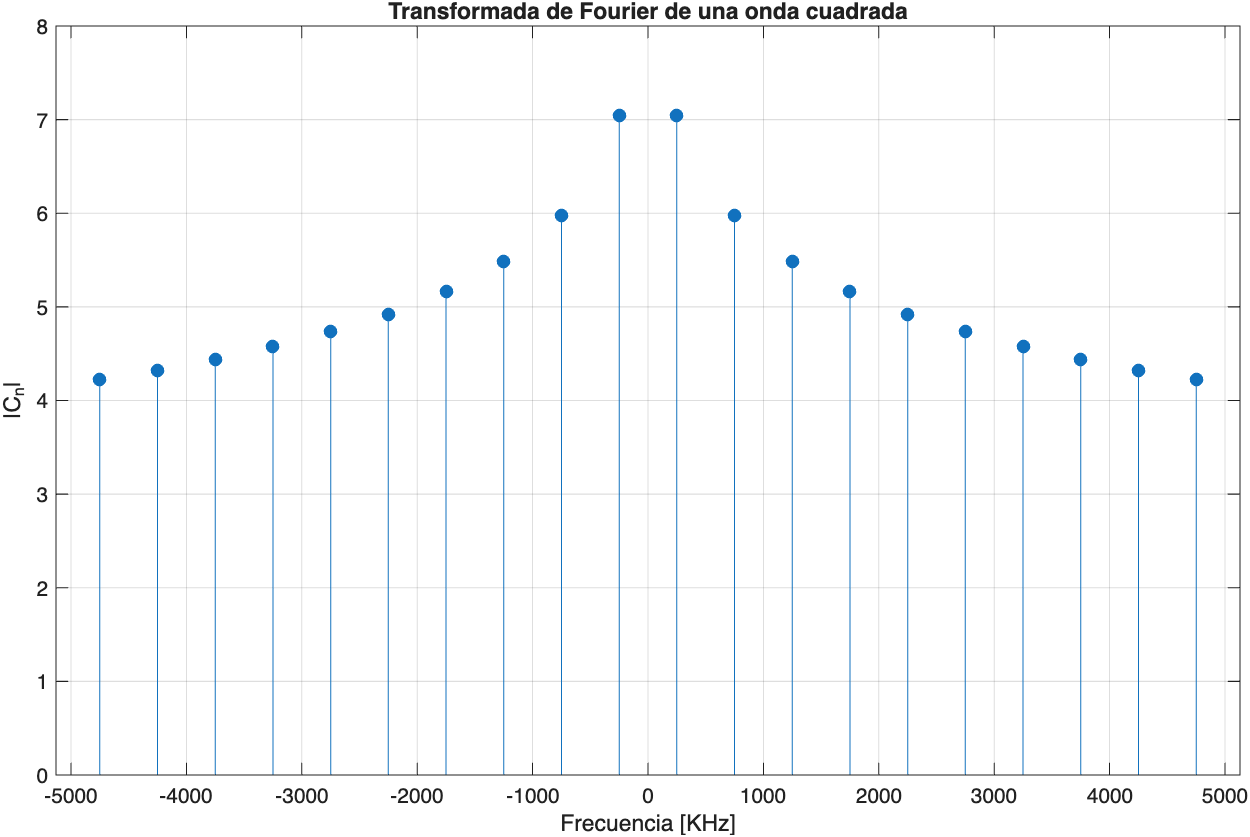
\includegraphics[width=0.8\textwidth]{FOTOS_TP6/simulaciones/TFcuadrada.png}
    \caption{Gráfico de la transformada de la función cuadrada con $f_0 = 250kHz$. Se graficó logaritmicamente en amplitud }
    \label{fig:TFCUADRADA}

    \end{minipage}
    \hfill
    %-------------------------
    %   FIGURA 2
    %-------------------------
    \begin{minipage}[b]{0.45\textwidth}
        \centering
    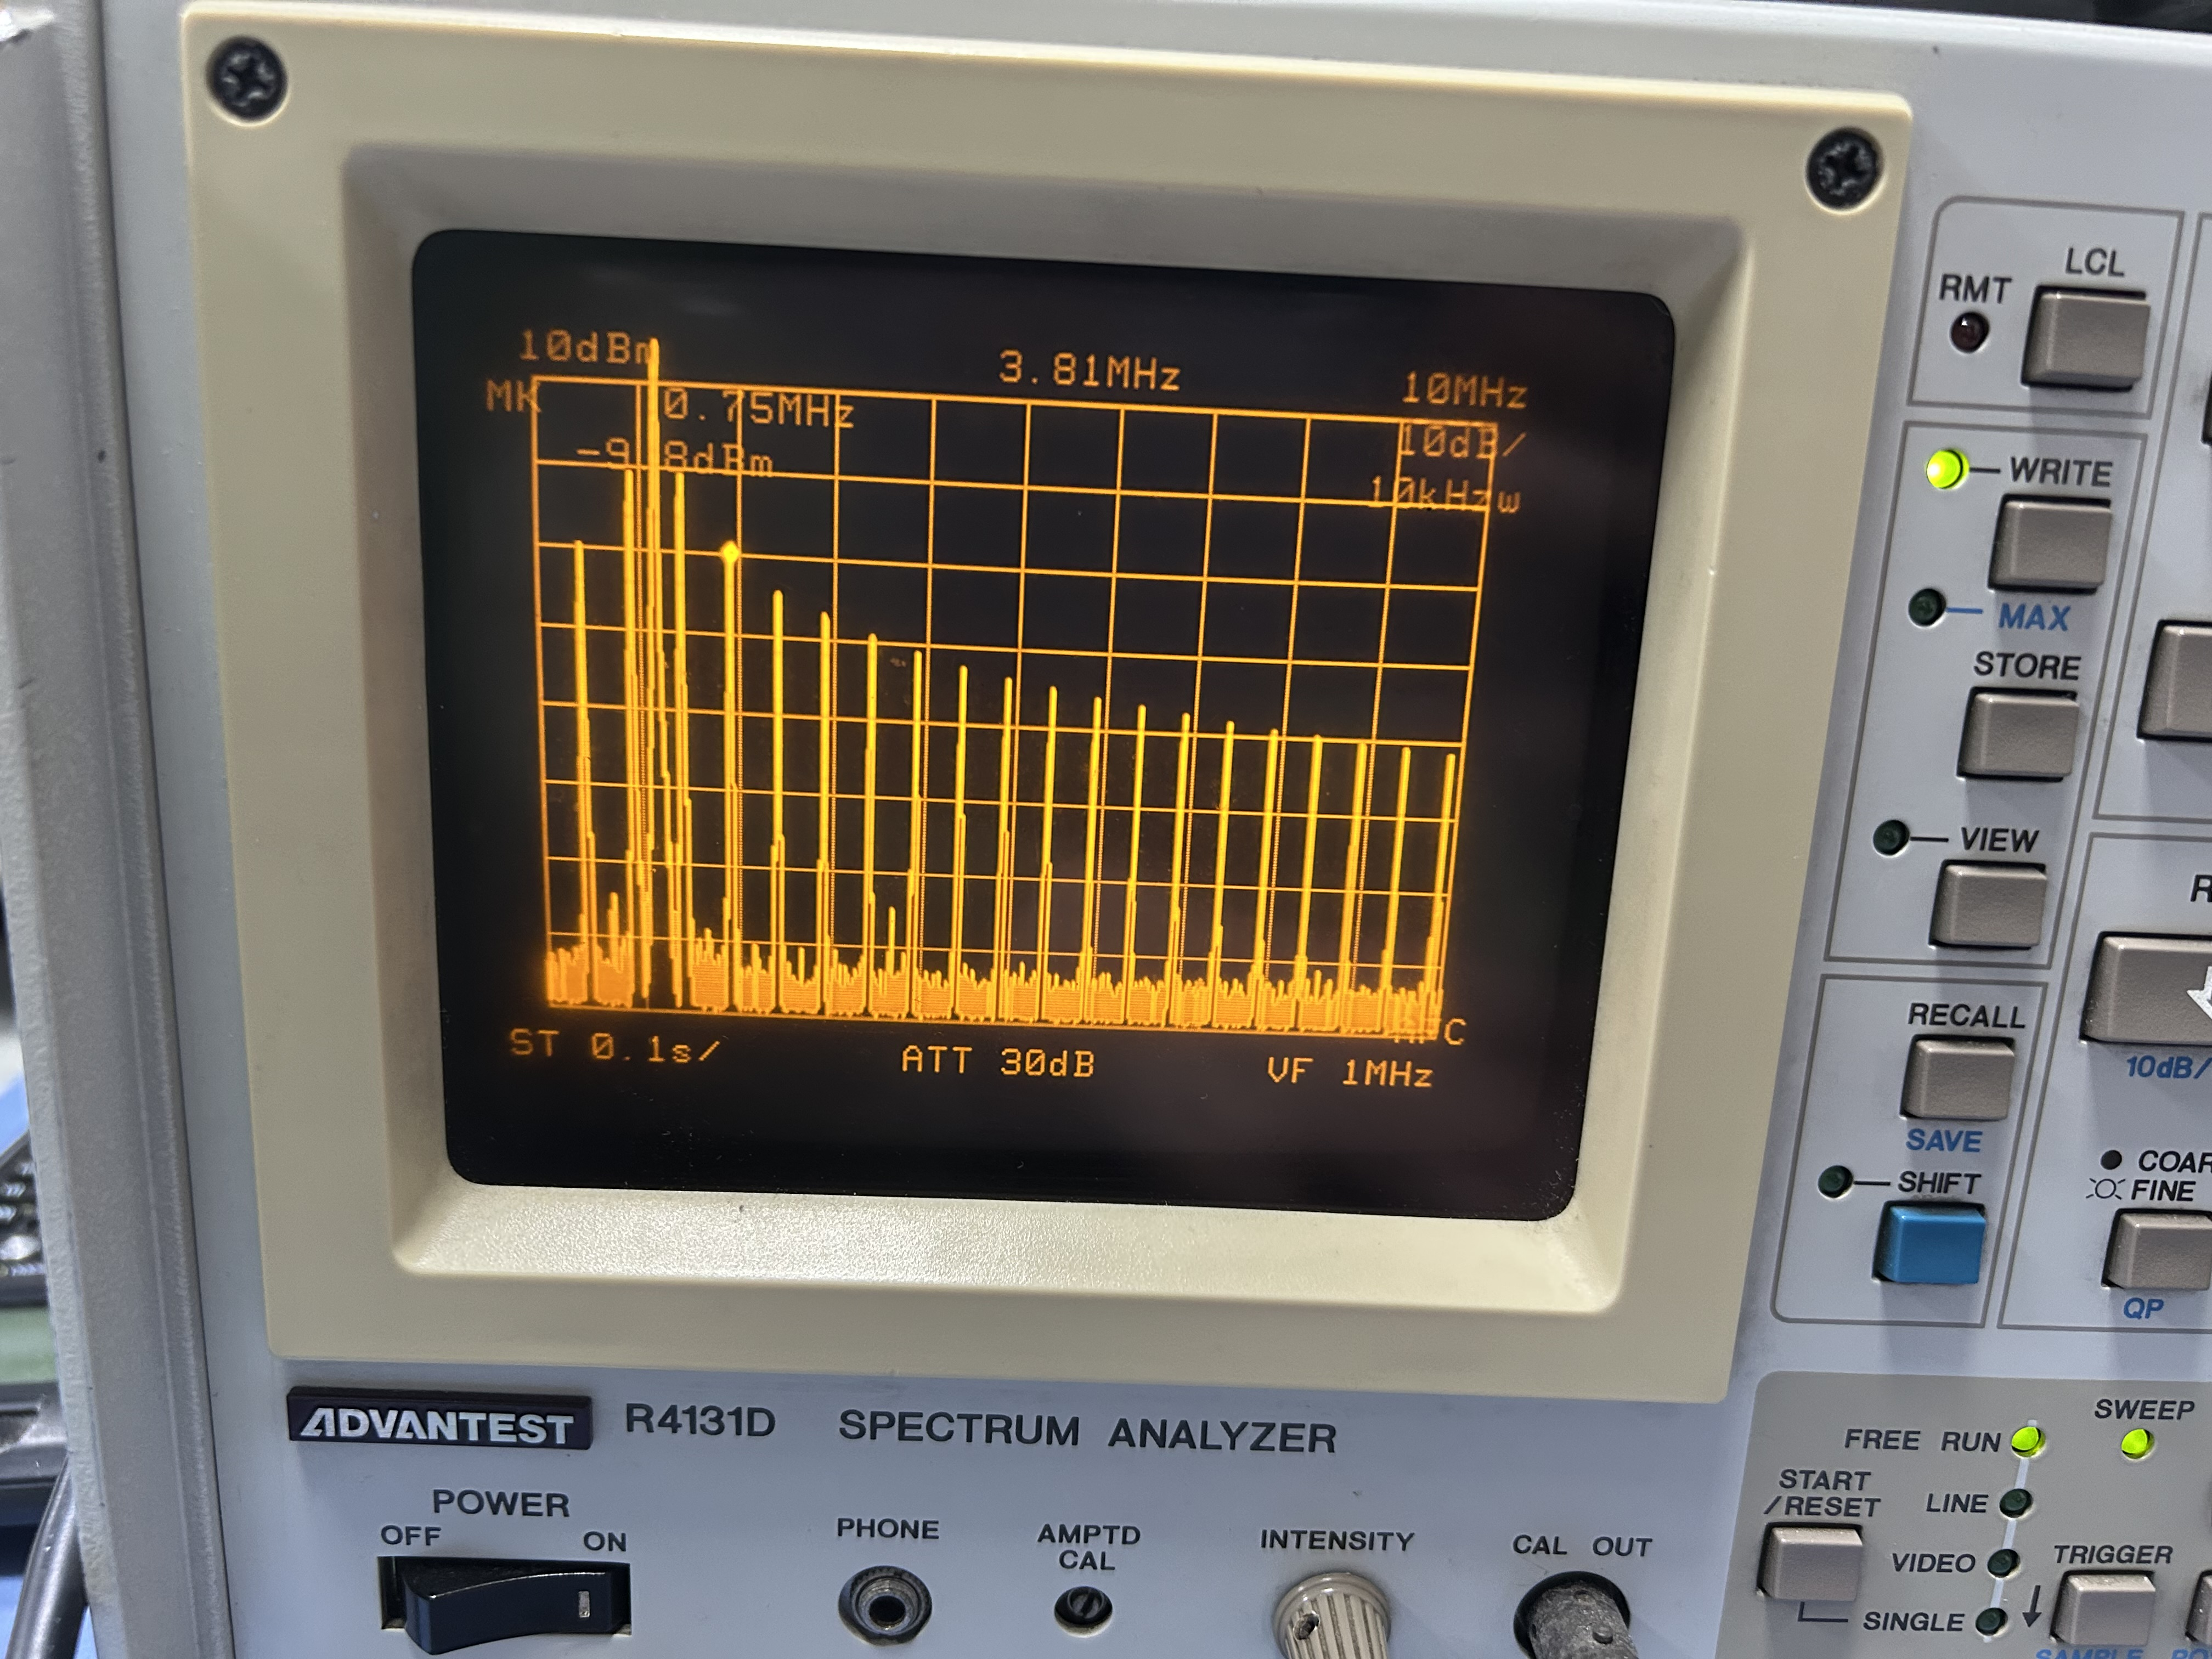
\includegraphics[width=0.8\textwidth]{FOTOS_TP6/PARTE 2/CUADRADA/IMG_8319.jpeg}
    \caption{Espectro de la señal cuadrada de 250KHz en el analizador de espectros}
    \label{fig:analizadoespectcuadrada}
    \end{minipage}

\end{figure}

Luego para el caso de una señal cuadrada de duty D se repite el procedimiento matemático:

\begin{equation}
\begin{aligned}
x(t)=
\left\{
\begin{matrix}
A & \text{si} & t\in(0,DT)\\
-A & \text{si} & t\in(DT,T)
\end{matrix}
\right.
\qquad\qquad
c_n=
\left\{
\begin{matrix}
A(2D-1), & n=0\\
2AD\,\mathrm{sinc}(nD)e^{-j\pi nD}, & n\neq0
\end{matrix}
\right.
\end{aligned}
\label{eq:coeficientrectangular}
\end{equation}

Finalmente, graficando se obtuvo la figura \ref{fig:TFRECT33} y se observó igual concordancia con lo medido en el analizador de espectro en la figura \ref{fig:analizadoespectrectangular}. Se puede observar en la figura y en la ecuación \ref{eq:coeficientrectangular}, que el Duty lo que hace es modelar cuales armónicos se anulan. En el caso del $D=\frac{1}{2}$ los armónicos que se anulan son todos los múltiplos de $\frac{1}{D}$, ósea los pares. Luego, en el caso de $D=\frac{1}{3}$, los armónicos anulados fueron los múltiplos de $\frac{1}{D}$.


\begin{figure}[h!]
    \centering

    %-------------------------
    %   FIGURA 1
    %-------------------------
    \begin{minipage}[b]{0.45\textwidth}
        \centering
    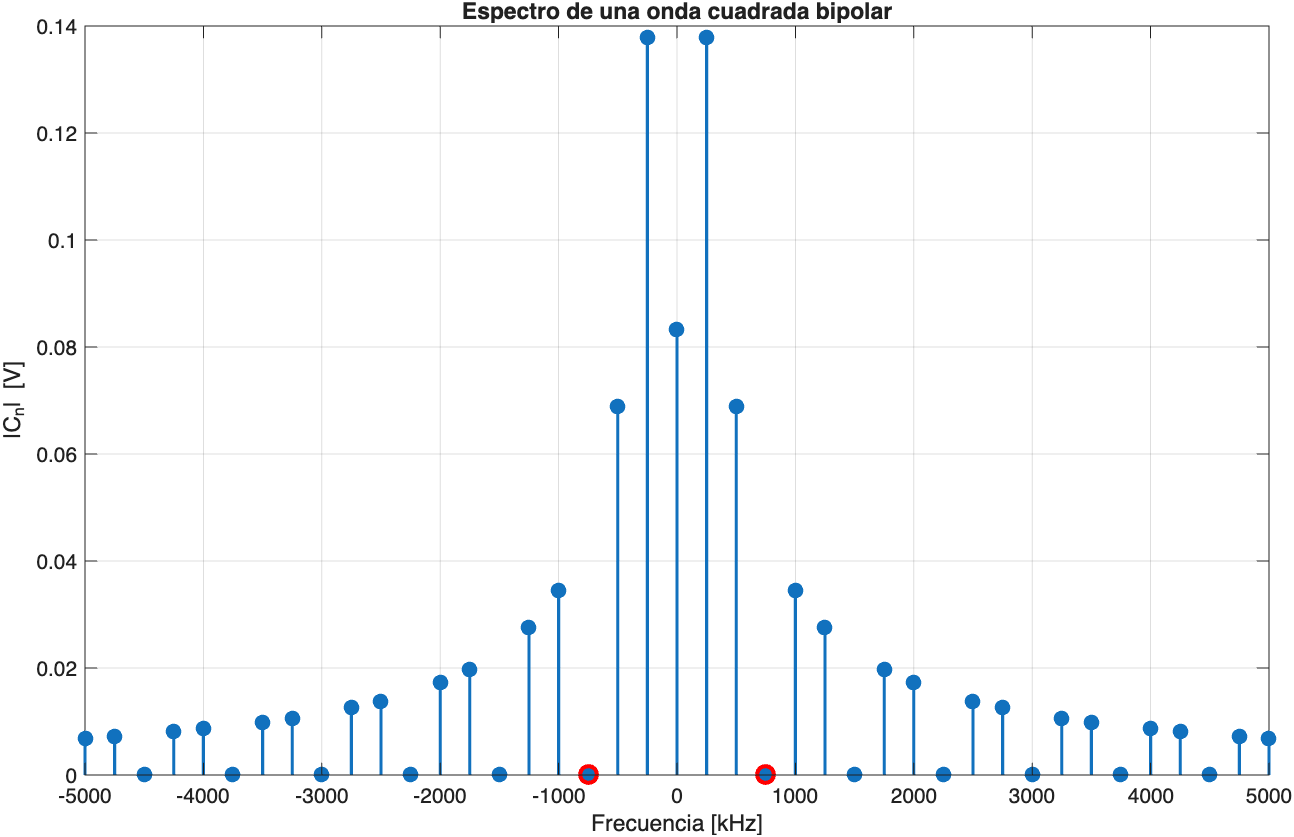
\includegraphics[width=0.8\textwidth]{FOTOS_TP6/simulaciones/TFcuadDuty33.png}
    \caption{Gráfico de la transformada de la función rectangular con $f_0 = 250kHz$ y D=0,33.}
    \label{fig:TFRECT33}

    \end{minipage}
    \hfill
    %-------------------------
    %   FIGURA 2
    %-------------------------
    \begin{minipage}[b]{0.45\textwidth}
        \centering
    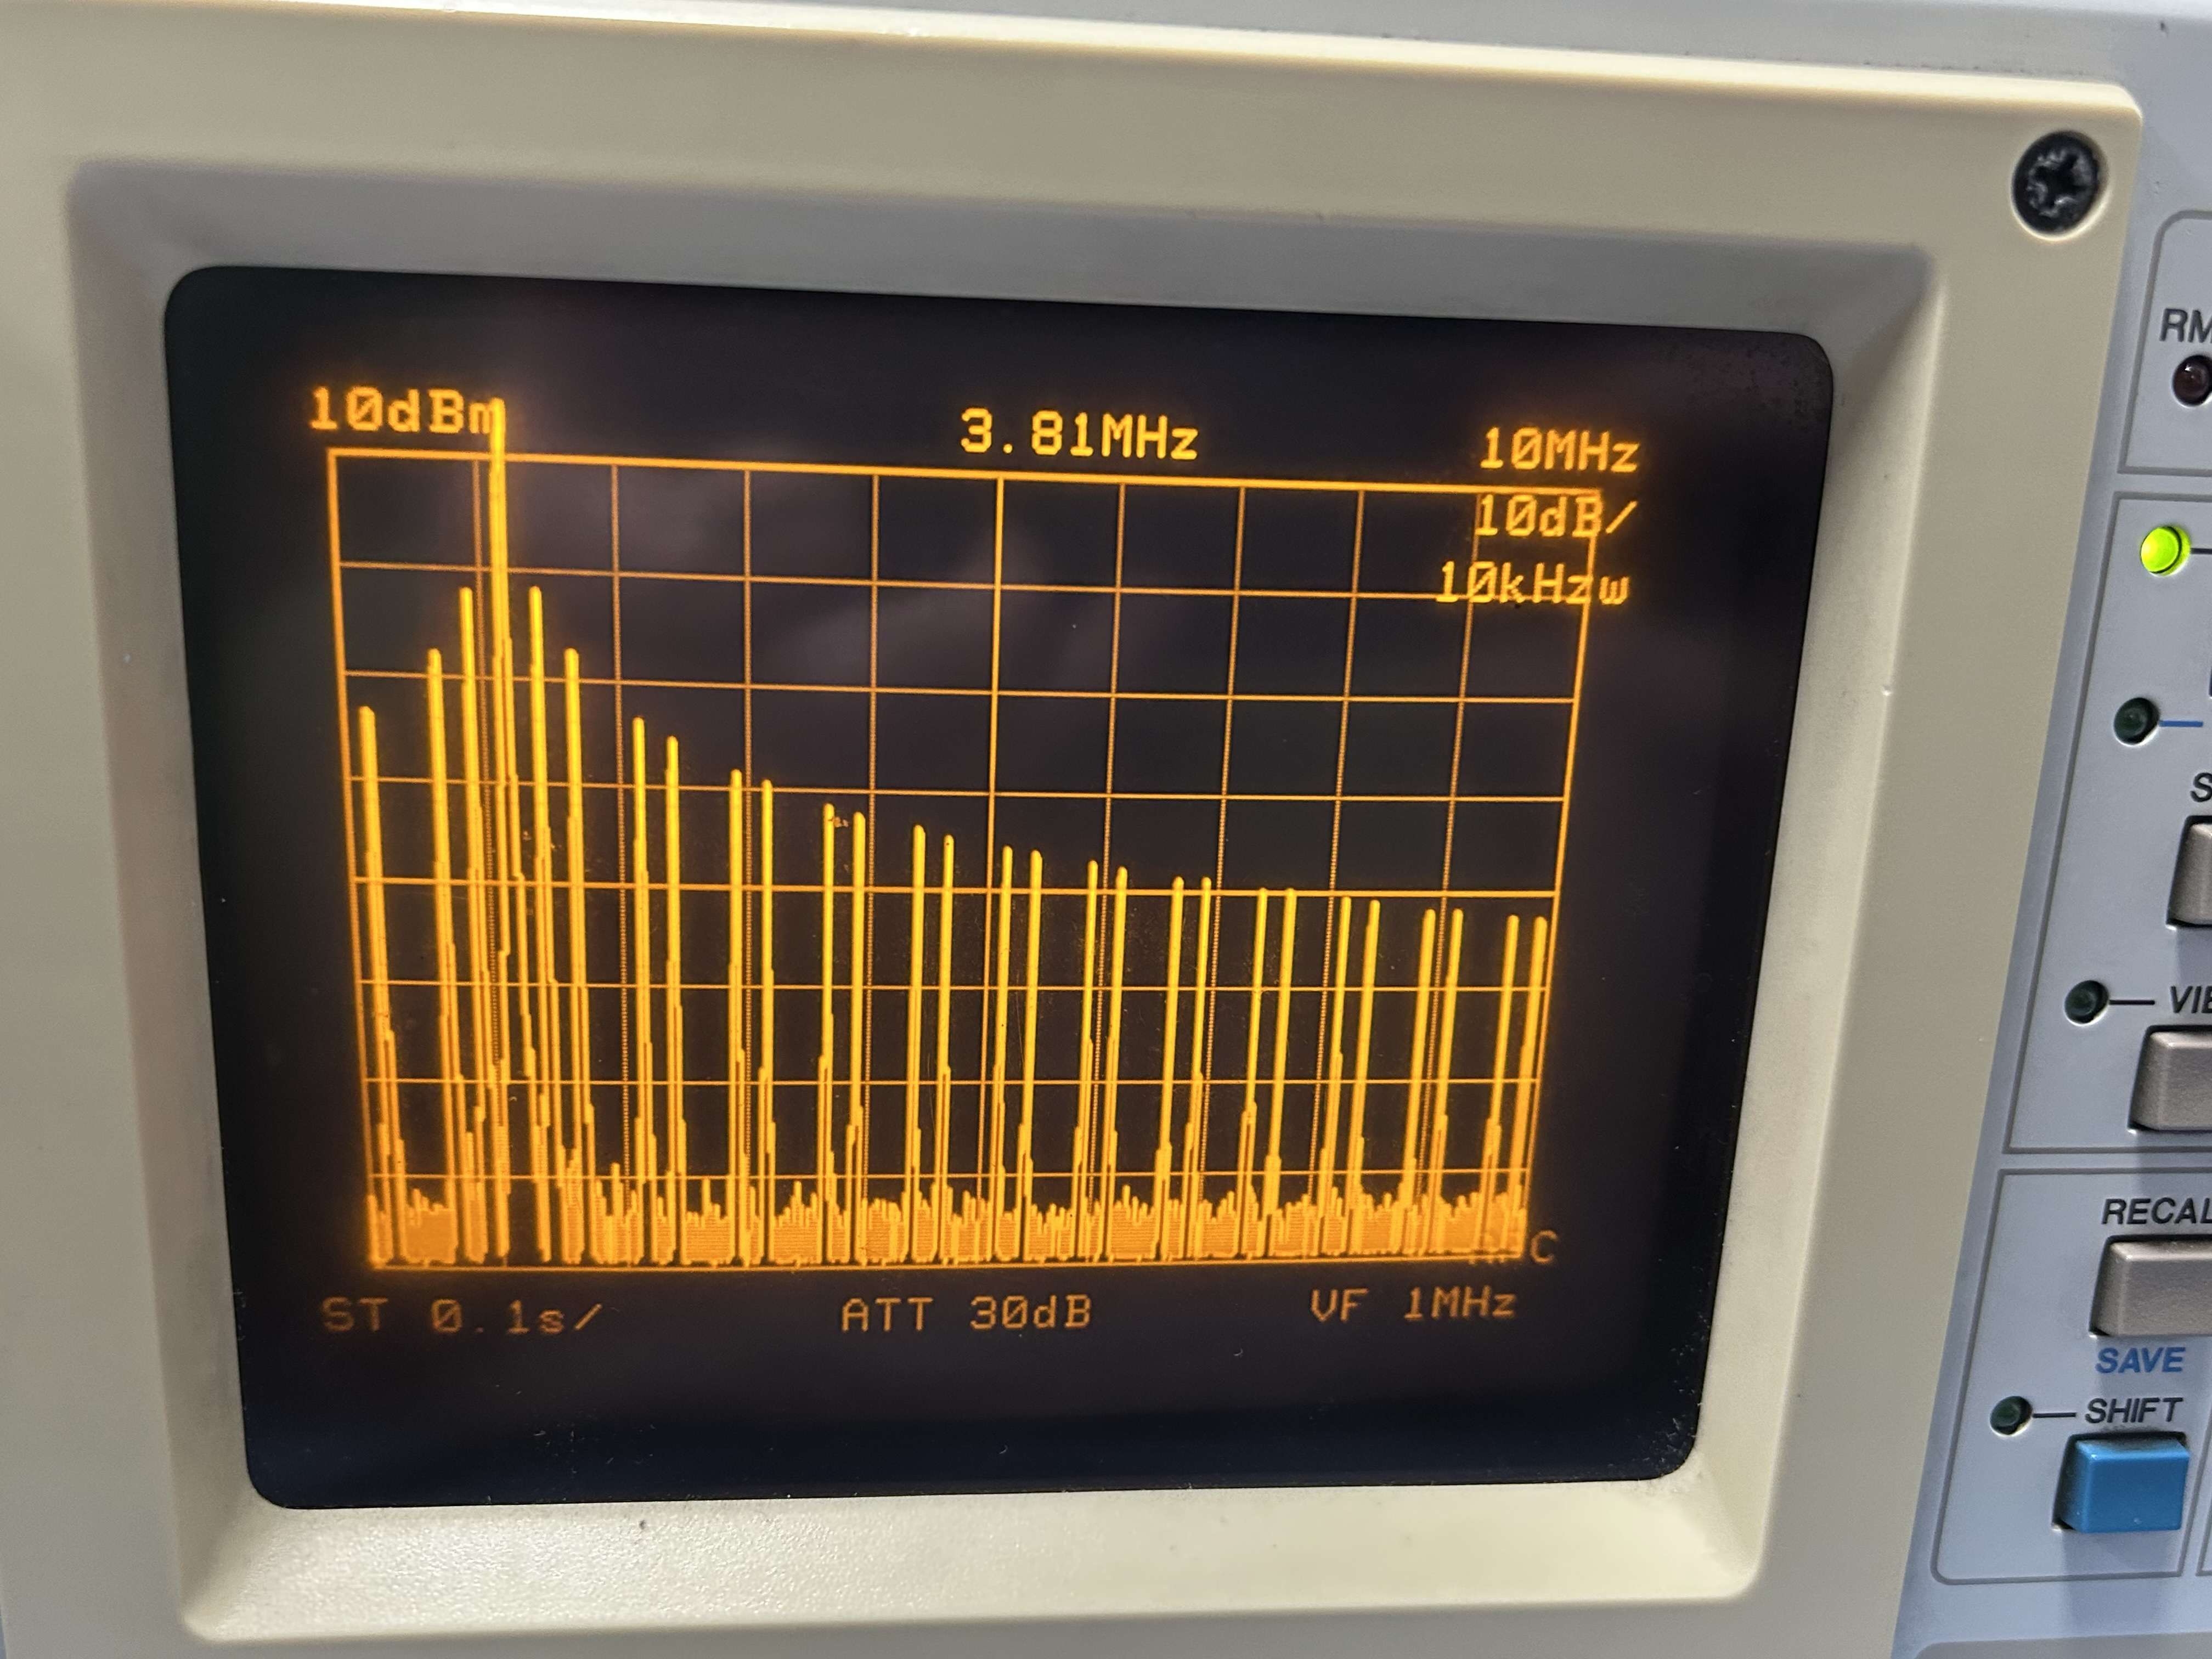
\includegraphics[width=0.8\textwidth]{FOTOS_TP6/PARTE 2/CUADRADA/IMG_8321.jpeg}
    \caption{Espectro de la señal rectangular de D=0,33 y $f_0 = 250KHz$ en el analizador de espectros}
    \label{fig:analizadoespectrectangular}
    \end{minipage}

\end{figure}

Finalmente, repitiendo el mismo procedimiento para una triangular se obtiene:

\begin{equation}
\begin{aligned}
x(t)=
\left\{
\begin{matrix}
\dfrac{4A}{T}t-A & \text{si} & t\in(0,\frac{T}{2})\\[6pt]
-\dfrac{4A}{T}t+3A & \text{si} & t\in(\frac{T}{2},T)
\end{matrix}
\right.
\qquad\qquad
c_n=
\left\{
\begin{matrix}
0, & n=0\\[6pt]
-\dfrac{2A}{\pi^2 n^2}\left(1-(-1)^n\right), & n\neq0
\end{matrix}
\right.
\end{aligned}
\label{eq:coeficienttriangular}
\end{equation}

Luego, se graficó la función en Matlab, y se graficó la amplitud en escala logarítmica (No se tuvo en cuenta la amplitud en el graficó de matlab, solo las frecuencias observadas) en la figura \ref{fig:TFtriang}. Luego se midió la salida del analizador de espectros en la figura \ref{fig:analizadoespectriang}. \par

Al comparar ambas imágenes, se observó una gran correlación en los armonicos vistos. En particular en este caso, la señal cumplió el mismo criterio dicho anteriormente del duty cicle, donde se anularon las frecuencias multiplos de $\frac{1}{D}$. Por tal motivo, se observaron las mismas frecuencias que en el caso de la cuadrada. No obstante, en este caso se observó, al comparar las figuras \ref{fig:analizadoespectrectangular} y \ref{fig:analizadoespectriang}, que los armónicos de la señal triangular se atenuaron mucho más rapidamente que los de la cuadrada. Esto se debe a que la cuadrada tiene cambios más bruscos que la triangular, por lo que los múltiplos de $c_n$ de los armónicos son mayores.

\begin{figure}[h!]
    \centering

    %-------------------------
    %   FIGURA 1
    %-------------------------
    \begin{minipage}[b]{0.45\textwidth}
        \centering
    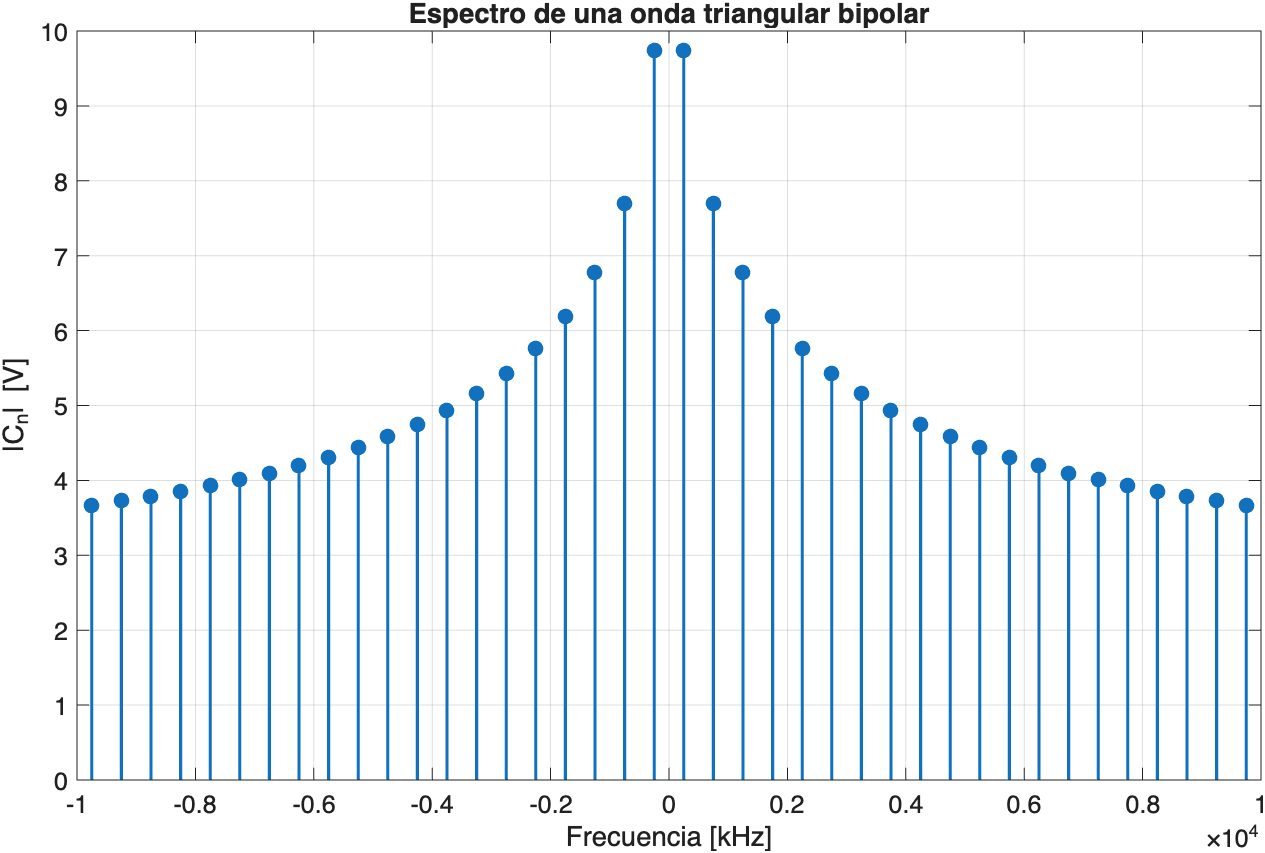
\includegraphics[width=0.8\textwidth]{FOTOS_TP6/simulaciones/TFtriangular.png}
    \caption{Gráfico de la transformada de la función triangular con $f_0 = 250kHz$ y D=0,5.}
    \label{fig:TFtriang}

    \end{minipage}
    \hfill
    %-------------------------
    %   FIGURA 2
    %-------------------------
    \begin{minipage}[b]{0.45\textwidth}
        \centering
    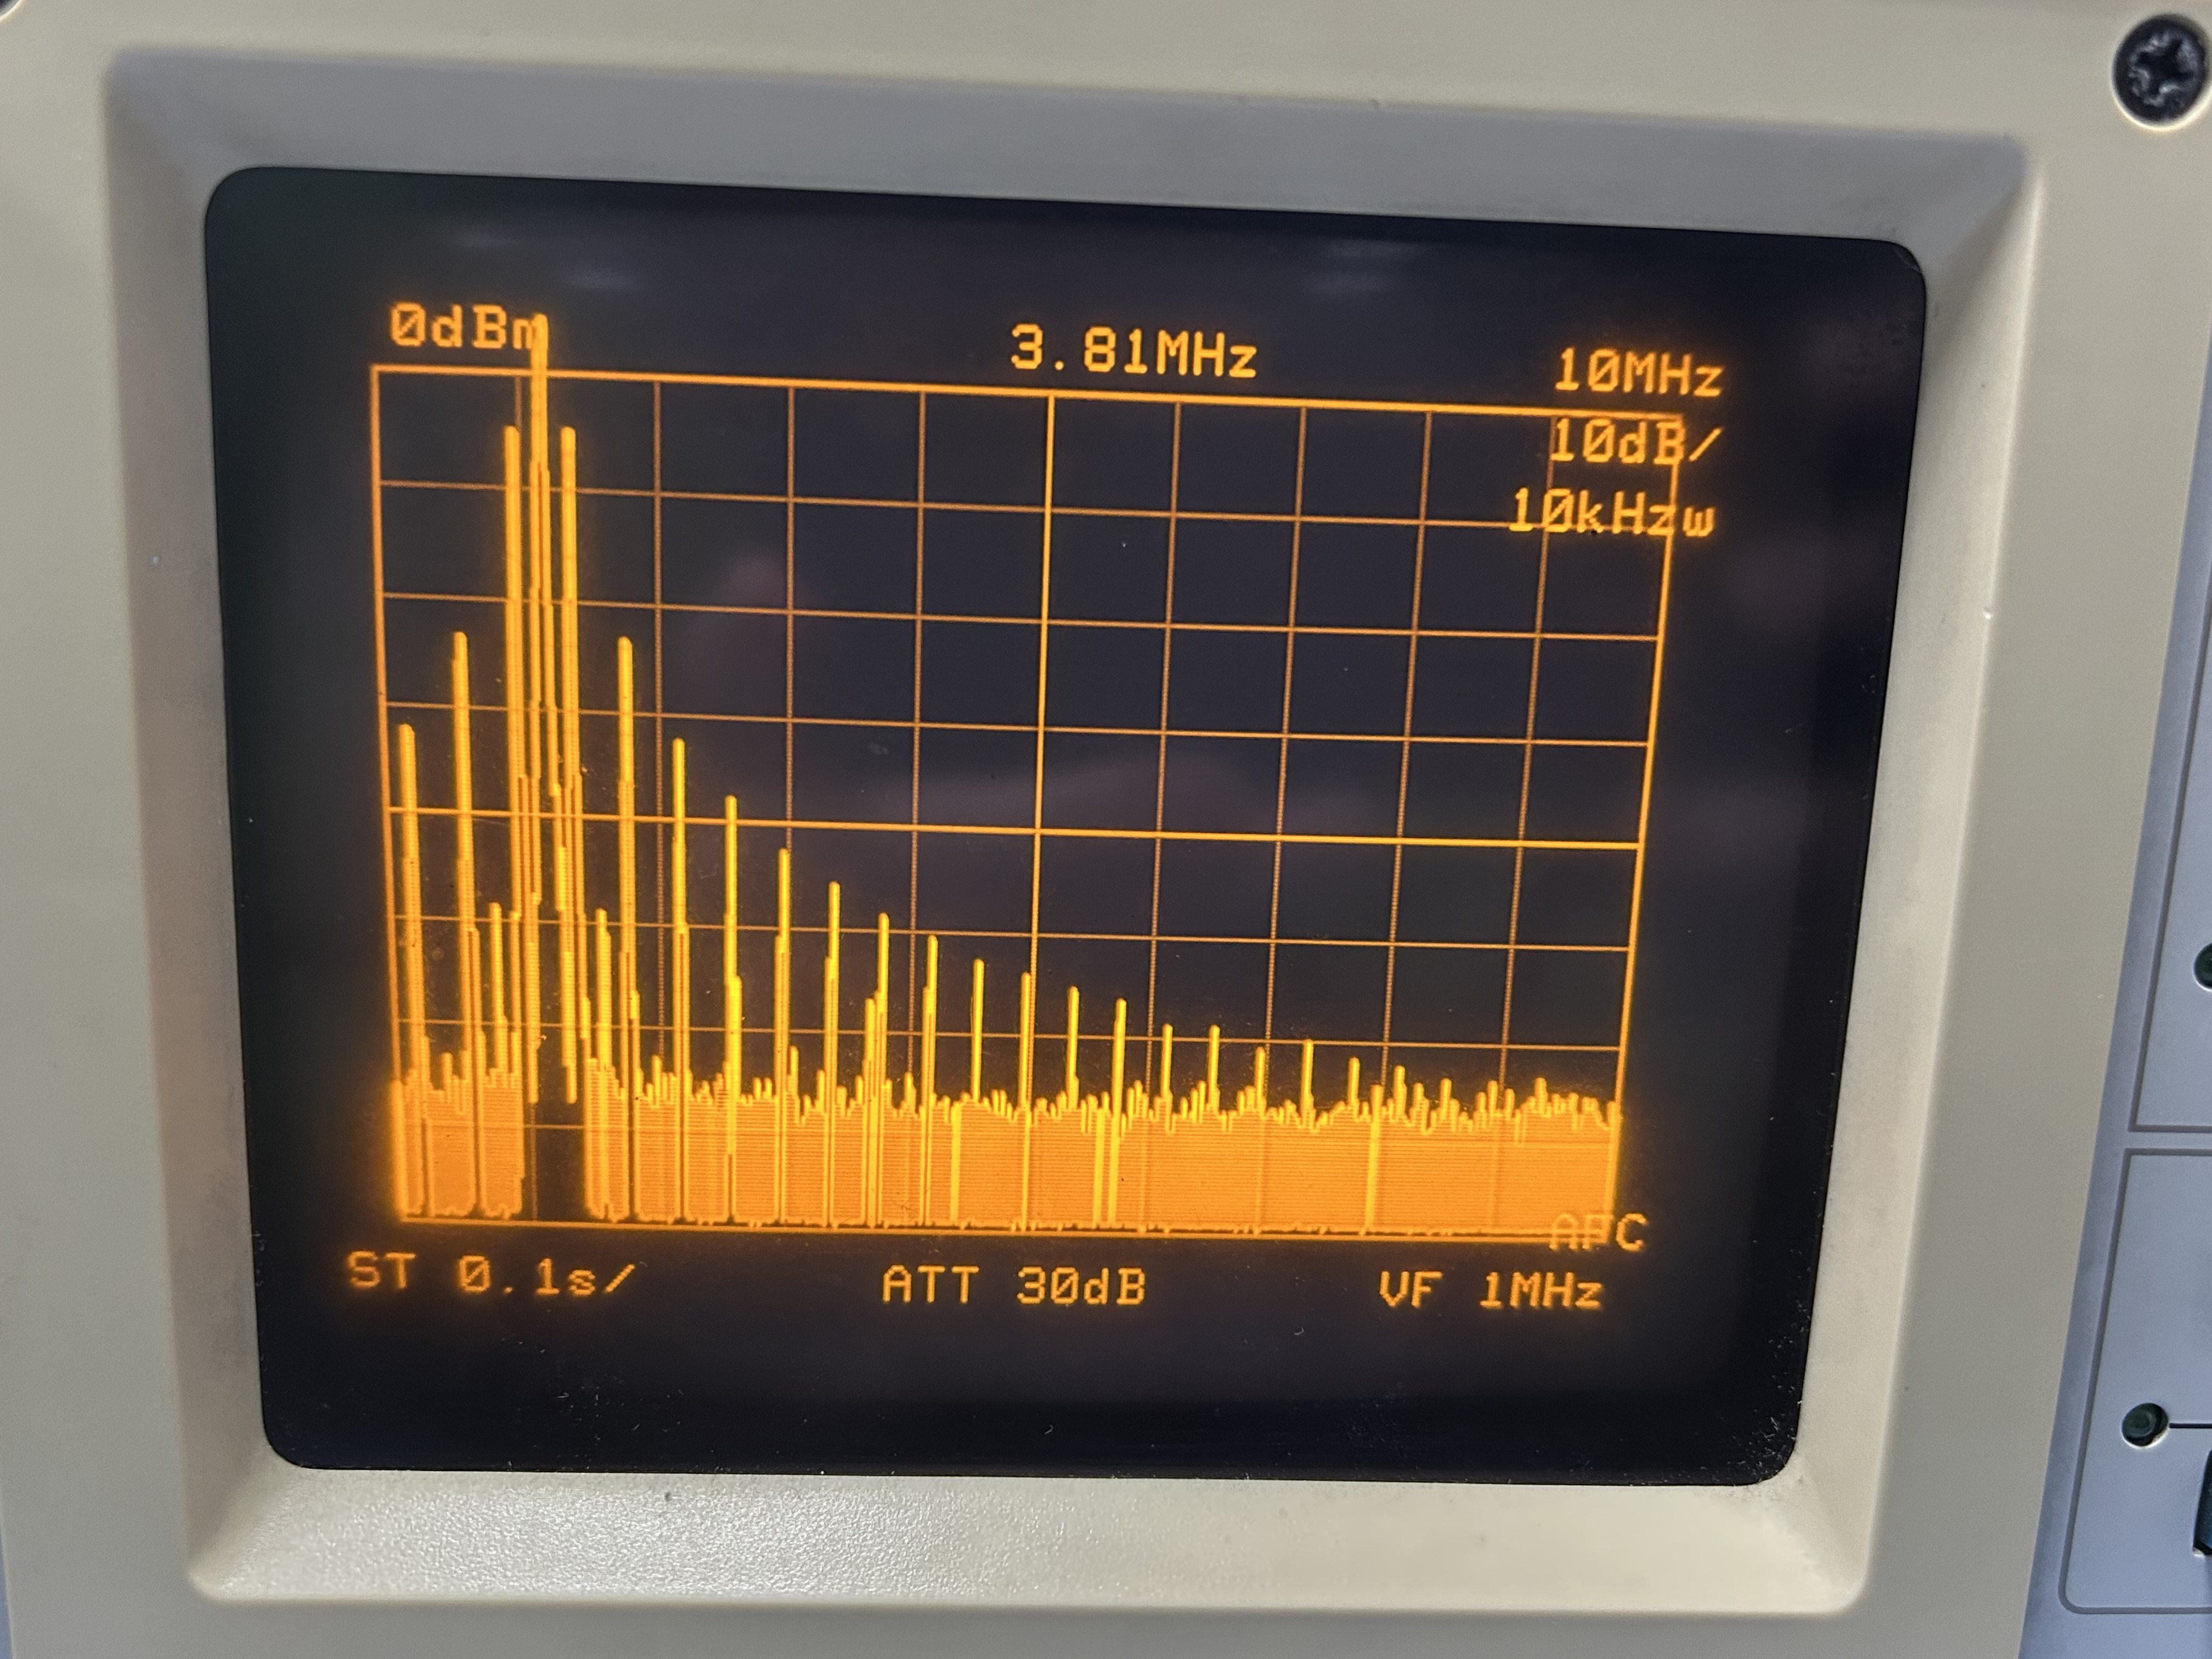
\includegraphics[width=0.8\textwidth]{FOTOS_TP6/PARTE 2/TRIANGULA/IMG_8323.jpeg}
    \caption{Espectro de la señal triangular de 250KHz en el analizador de espectros}
    \label{fig:analizadoespectriang}
    \end{minipage}

\end{figure}







